\documentclass[11pt,a4paper]{article}

\usepackage[margin=2.5cm]{geometry}
\usepackage{graphicx}
\usepackage[space]{grffile}   % allows spaces in image filenames
\usepackage{hyperref}
\usepackage{listings}
\usepackage{xcolor}
\usepackage{booktabs}
\usepackage{caption}
\usepackage{parskip}
\usepackage{float}   % provides [H] float placement (exactly here, no drift)

\hypersetup{
    colorlinks=true,
    linkcolor=blue!60!black,
    urlcolor=blue!60!black,
}

\lstdefinestyle{shell}{
    backgroundcolor=\color{gray!10},
    basicstyle=\ttfamily\small,
    breaklines=true,
    frame=single,
    framerule=0.4pt,
    rulecolor=\color{gray!50},
    xleftmargin=1em,
    xrightmargin=1em,
}
\lstset{style=shell}

\title{\textbf{PyAutoRoute Tutorial}\\[0.4em]
       \large An introduction to PyAutoRoute}
\author{D. Q. McDonald}
\date{}

\begin{document}

\maketitle

\begin{center}
    \fbox{\parbox{0.85\textwidth}{\centering
        \textbf{Note:} This tutorial is a work in progress.
        Some sections may be incomplete or subject to change.
    }}
\end{center}

\tableofcontents
\newpage

% -----------------------------------------------------------------------
\section{Introduction}

PyAutoRoute is a Python tool that automatically places and routes
two-layer KiCad PCBs without requiring the \texttt{pcbnew} Python
bindings --- it reads and writes the \texttt{.kicad\_pcb} s-expression
format directly, so it runs in any normal Python environment.

Given a board with footprints placed and nets assigned, PyAutoRoute
produces a routed copy that is DRC-clean by construction: clearance to
other tracks, pads, vias, and the board edge is enforced on an
inflated routing grid, so the router can never produce a short or a
clearance violation.

It can also \emph{place} the footprints automatically before routing,
using a simulated-annealing pass that minimises rats-nest length while
keeping component bodies apart.

This tutorial walks through routing a small but realistic board: a
selectable-clock circuit for a Z80 retrocomputer, offering three clock
sources controlled by a jumper.

% -----------------------------------------------------------------------
\section{The Tutorial Circuit}

The first stage is to create a schematic. For this tutorial we'll be using
a circuit (Figure~\ref{fig:schematic}) that implements three clock
sources for a Z80-based computer:

\begin{enumerate}
    \item \textbf{555 Timer clock} --- a \textsc{TLC555xP} astable
          oscillator whose frequency is set by a potentiometer
          (\texttt{RV1}) and timing capacitors.
    \item \textbf{4\,MHz crystal oscillator} --- a Pierce oscillator
          built from two \textsc{74HC14} Schmitt-trigger inverters and
          a 4\,MHz crystal (\texttt{Y1}).
    \item \textbf{Manual (single-step) clock} --- a debounced
          pushbutton (\texttt{SW1}) for stepping through instructions
          one cycle at a time.
\end{enumerate}

\begin{figure}[H]
    \centering
    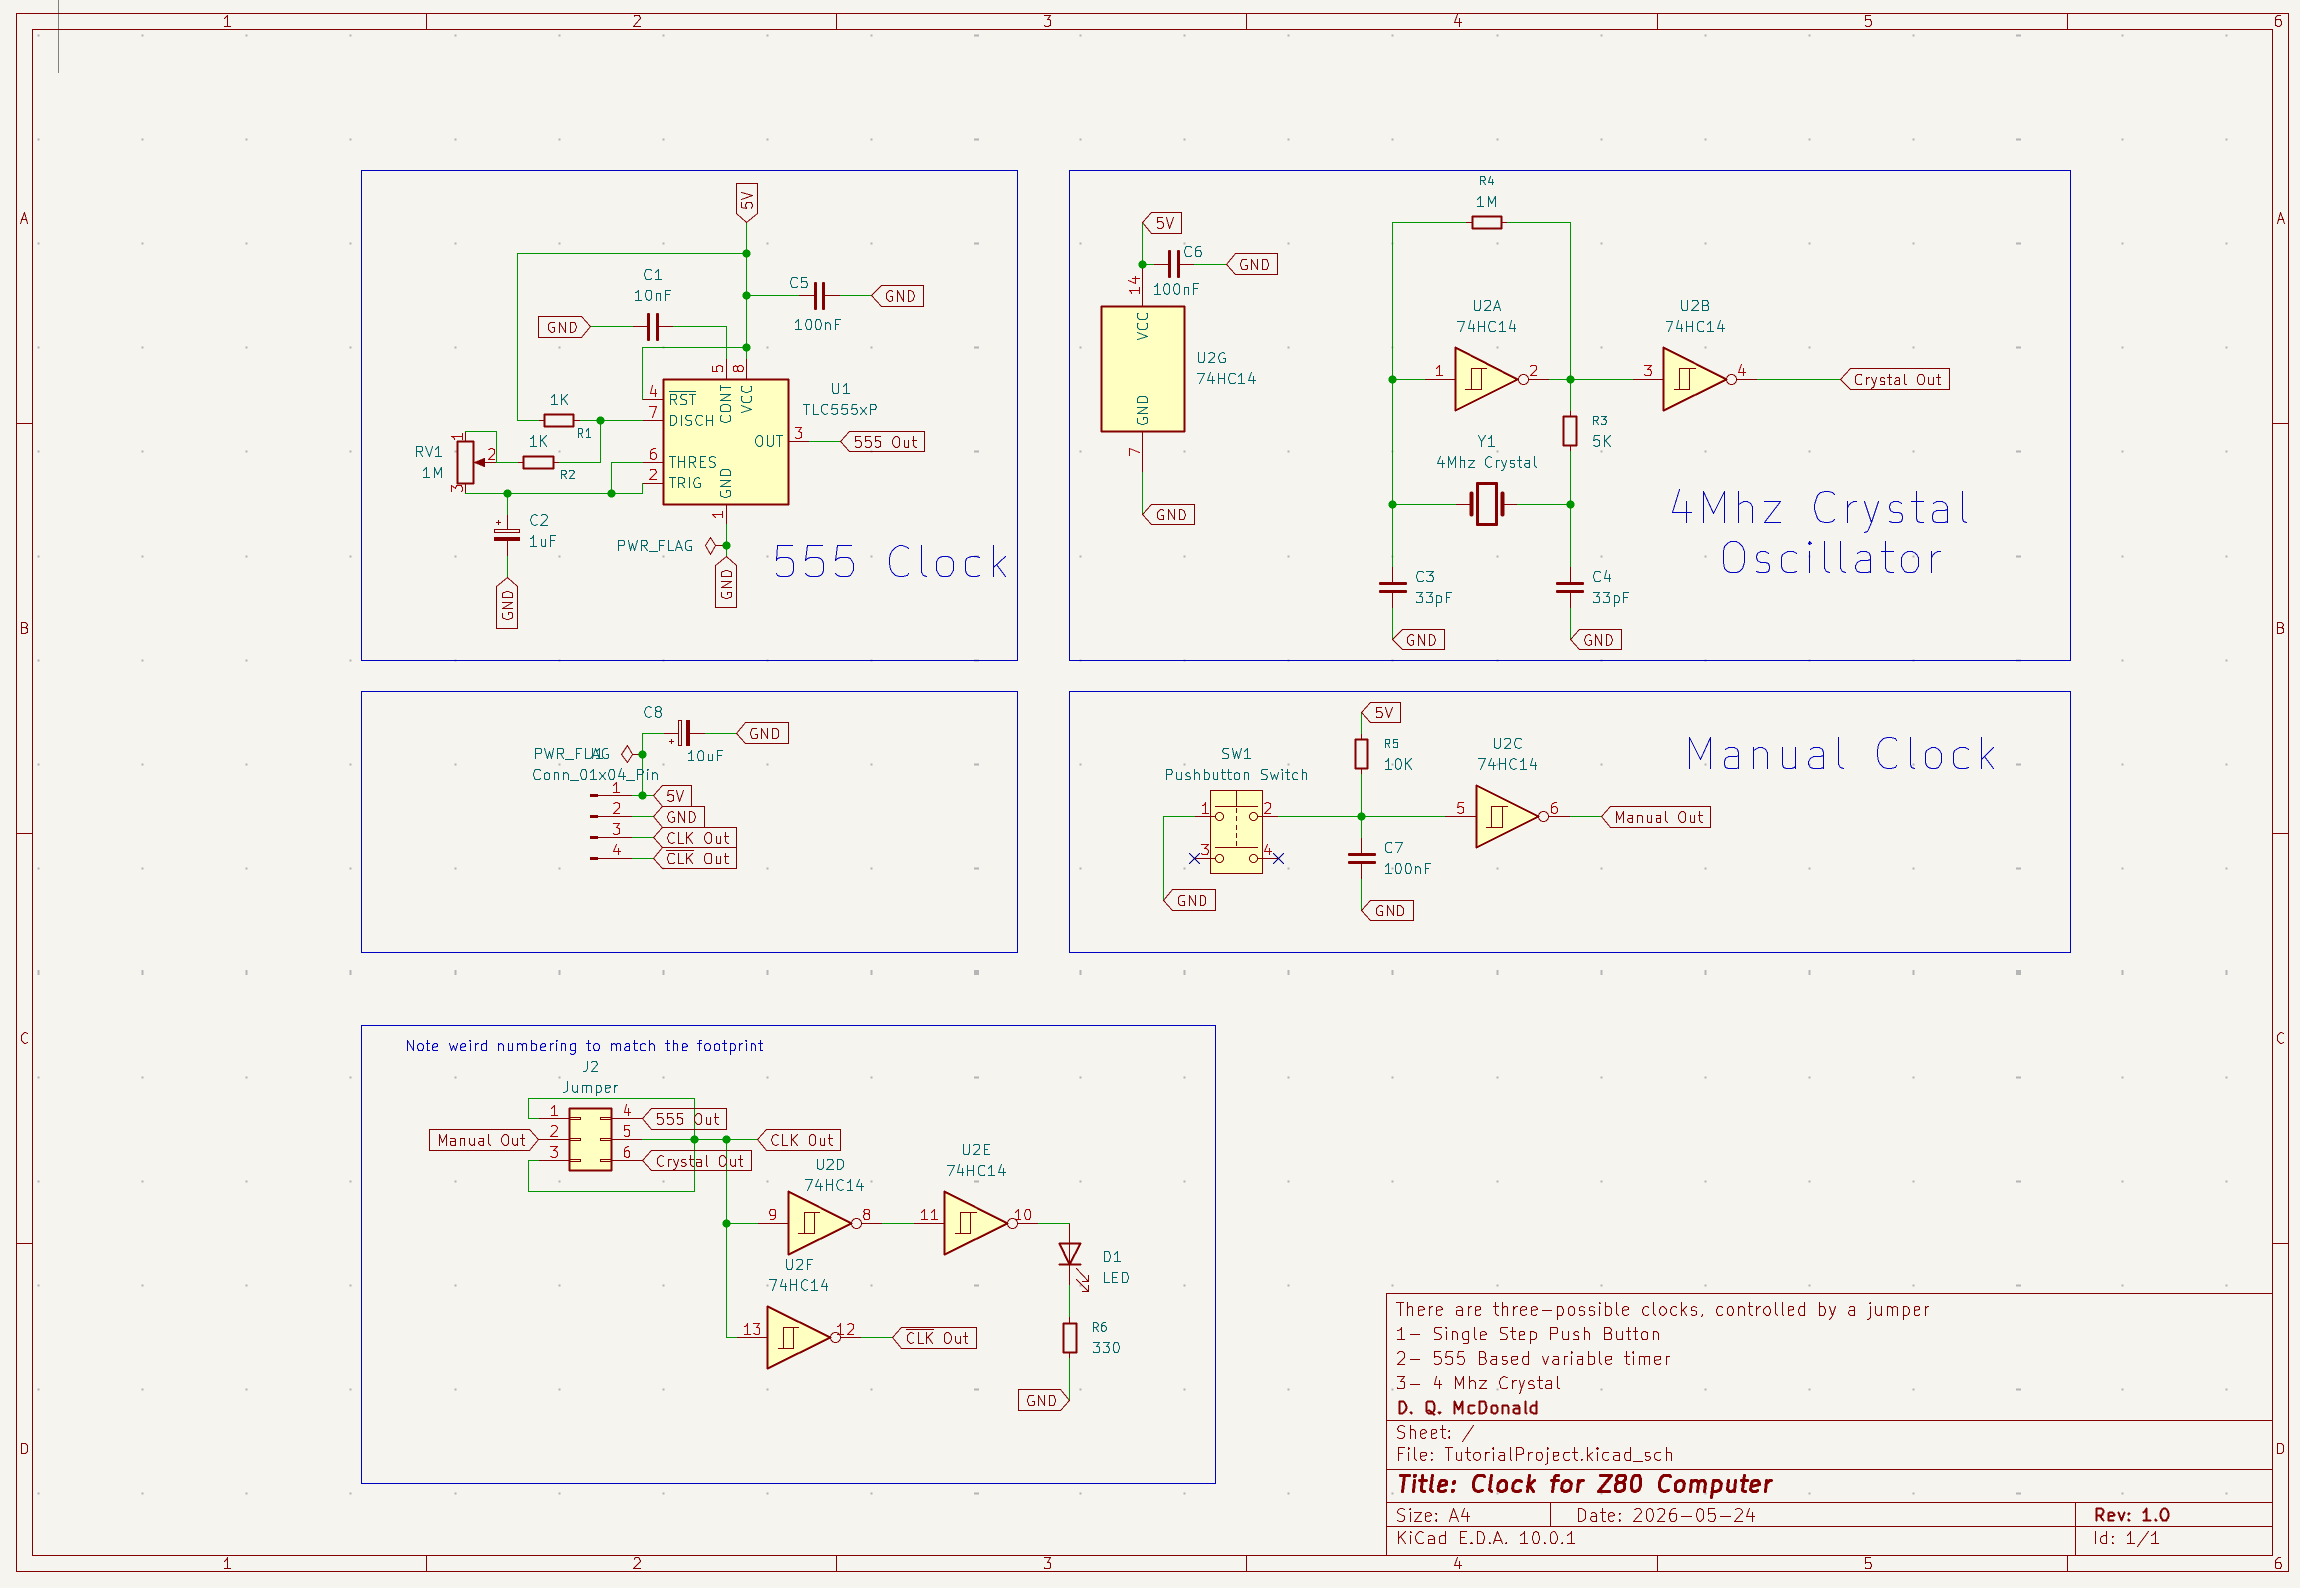
\includegraphics[width=\textwidth]{images/Schematic.png}
    \caption{KiCad schematic --- Clock for Z80 Computer.}
    \label{fig:schematic}
\end{figure}

Once your schematic is complete you should use the Electrical Rules Check to ensure
that it is complete. Then you can assign footprints using the built-in tool in KiCad. 
This can also be a tiresome task and the next section describes a tool that provides some
help with automating that. 

\subsection*{Assigning footprints with \texttt{pyautoroute-assign}}

Before a schematic can be turned into a PCB layout, every symbol needs a
\emph{footprint} --- the physical land pattern that will be manufactured
on the board. PyAutoRoute includes a companion tool,
\texttt{pyautoroute-assign}, that fills in empty \texttt{Footprint}
fields in a \texttt{.kicad\_sch} file automatically, using a personal
preference database you configure once.

Footprints are assigned by component prefix (\texttt{R}, \texttt{C},
\texttt{CP}, \texttt{U}, \ldots) and, for ICs, by the symbol's
\texttt{Value} field. A quick preview before any file is written is
available with \texttt{--dry-run}:

\begin{lstlisting}
# Preview what would be assigned
pyautoroute-assign TutorialProject.kicad_sch --dry-run

# Assign footprints using your preferences
pyautoroute-assign TutorialProject.kicad_sch
\end{lstlisting}

On first use, run \texttt{--init-prefs} to create the preference file and
\texttt{--rebuild-index} to scan your KiCad library. See the
\emph{Assigning footprints} section of the \texttt{README} for the full
option reference.


% -----------------------------------------------------------------------
\section{Prerequisites}

\begin{itemize}
    \item \textbf{KiCad 6 or later} --- to view and edit the schematic
          and PCB files.
    \item \textbf{Python 3.10+} with \texttt{numpy}, \texttt{scipy},
          and \texttt{shapely $\geq$ 2.0}.
    \item \textbf{PyAutoRoute} installed:
\begin{lstlisting}
pip install -e /path/to/PyAutoRoute
\end{lstlisting}
    \item The tutorial project files in the \texttt{TutorialProject/}
          subdirectory alongside this document.
\end{itemize}

Verify the installation:

\begin{lstlisting}
pyautoroute --version
\end{lstlisting}

% -----------------------------------------------------------------------
\section{Starting Point: the Unrouted Board}

Open \texttt{TutorialProject/TutorialProject.kicad\_pcb} in KiCad.
You will see the footprints arranged roughly in functional groups
(Figure~\ref{fig:initial}), with thin \emph{ratsnest} lines indicating
the connections that need to be routed.

\begin{figure}[H]
    \centering
    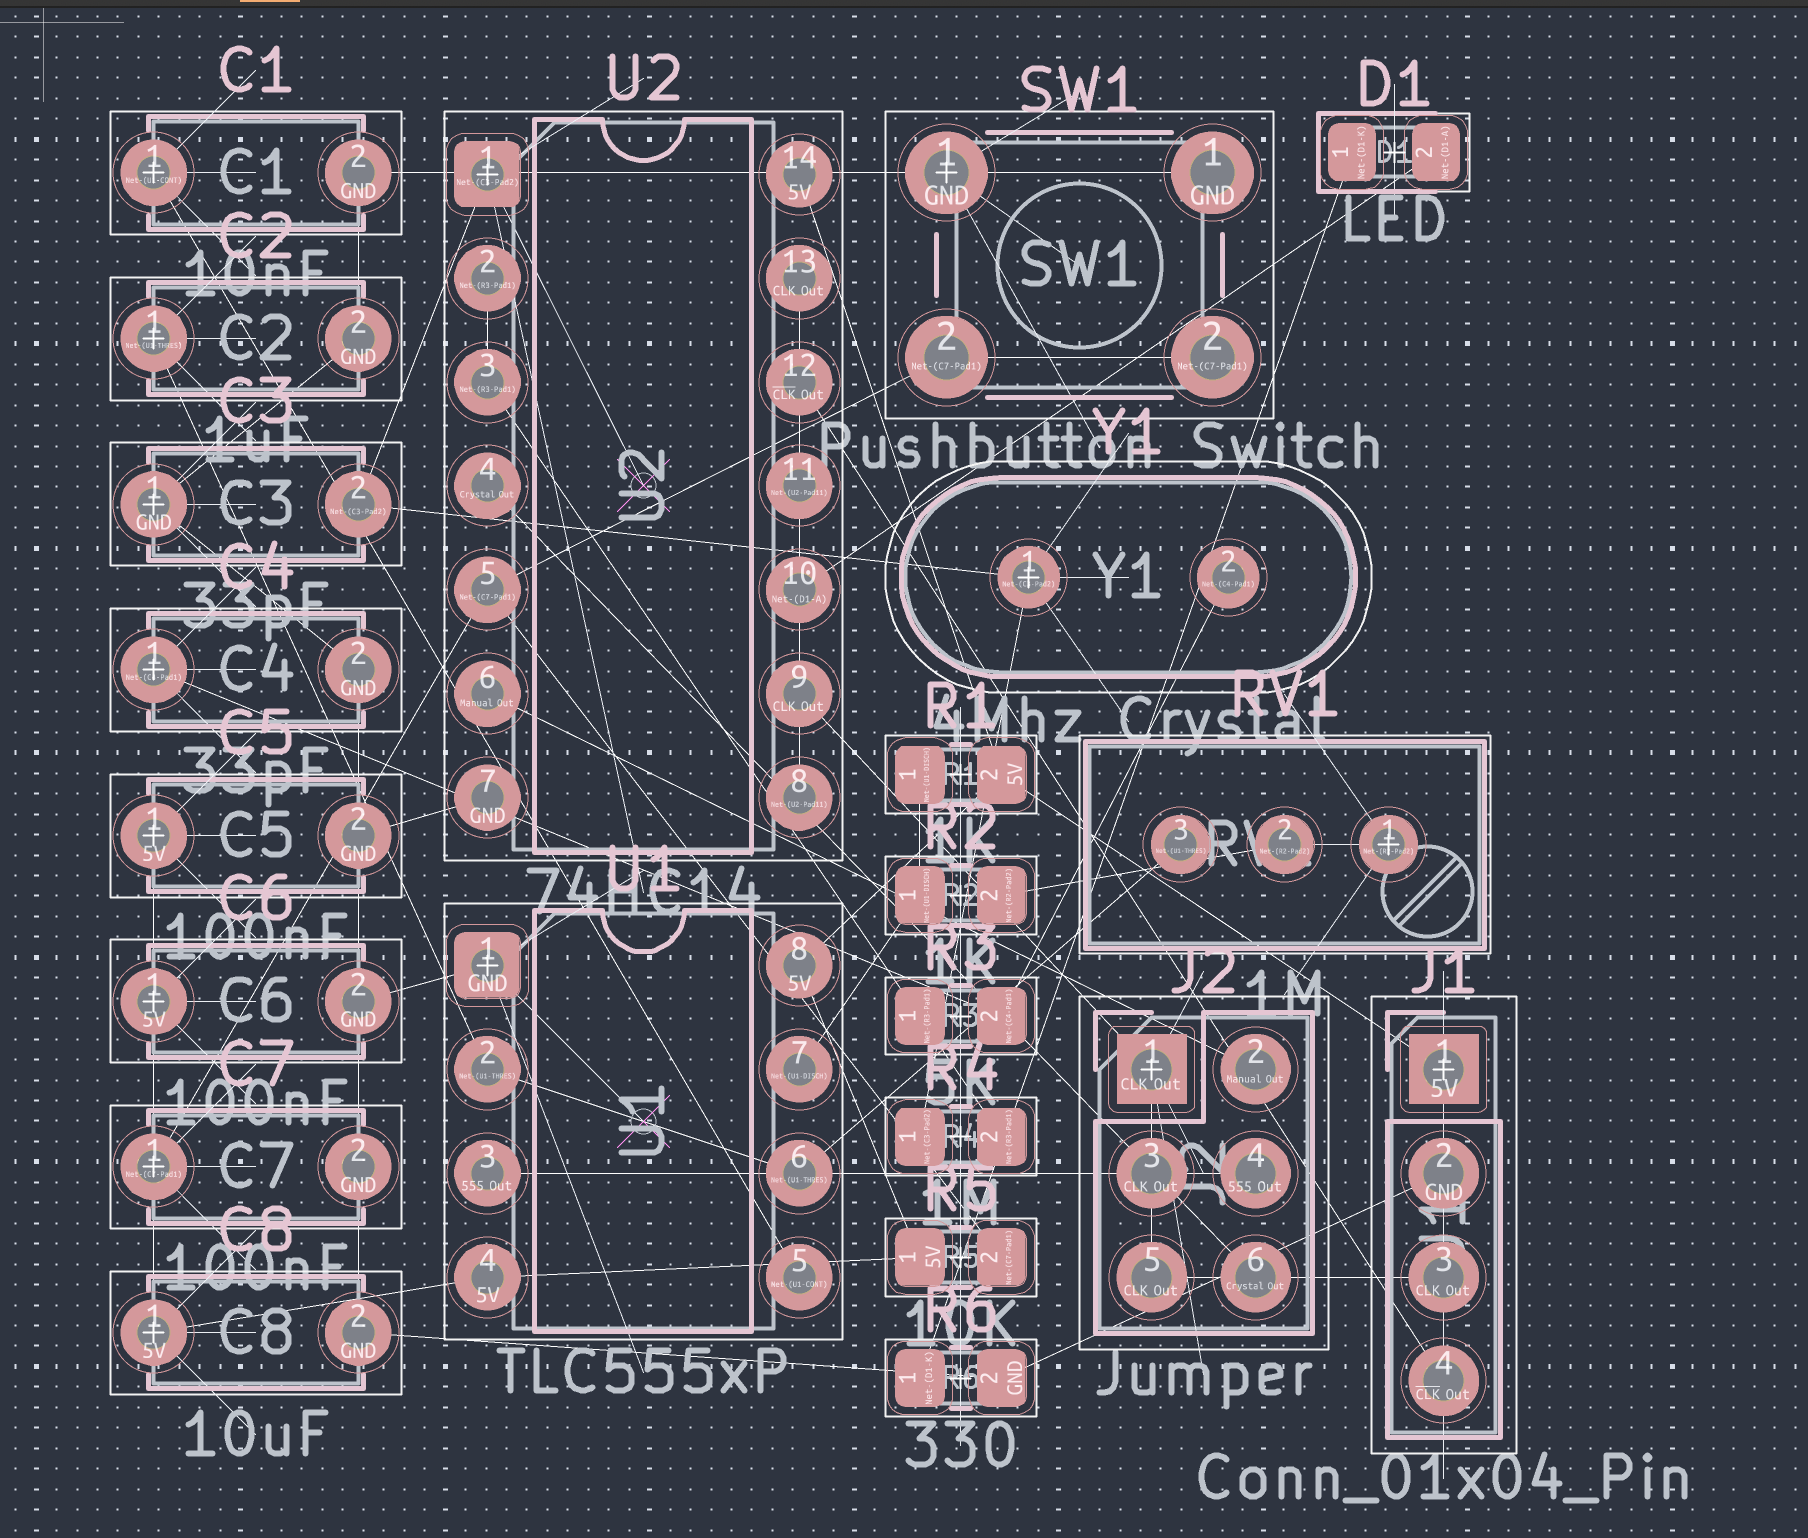
\includegraphics[width=0.85\textwidth]{images/Initial PCB Layout.png}
    \caption{Initial PCB layout --- footprints placed, no tracks yet.
             The pink lines are the ratsnest (unrouted connections).}
    \label{fig:initial}
\end{figure}

At this stage:
\begin{itemize}
    \item All footprints have been placed manually in approximate
          functional groups.
    \item Nets are assigned (exported from the schematic via
          \emph{File $\to$ Export $\to$ Netlist}).
    \item No tracks exist yet --- the board is purely a placed netlist.
\end{itemize}

% -----------------------------------------------------------------------
\section{Adding a Board Outline}

Before routing, KiCad needs an \texttt{Edge.Cuts} outline so the
router knows the board boundary. Figure~\ref{fig:border} shows the
board after a rectangular outline has been drawn around the components.

\begin{figure}[H]
    \centering
    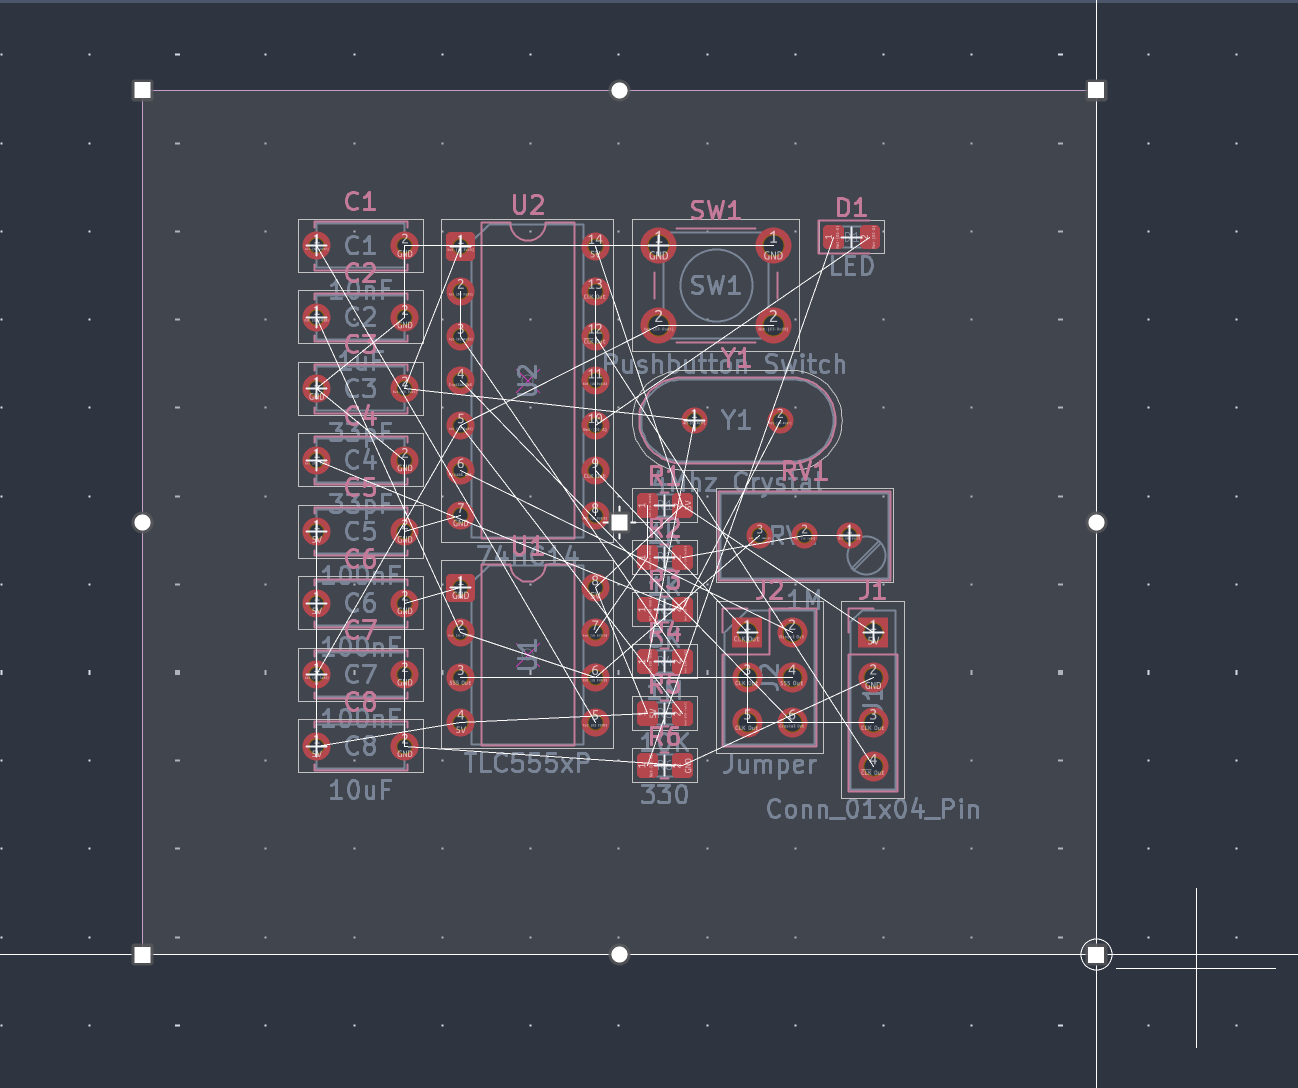
\includegraphics[width=0.75\textwidth]{images/Boarder.png}
    \caption{Board with \texttt{Edge.Cuts} outline added. PyAutoRoute
             keeps all tracks inside this boundary.}
    \label{fig:border}
\end{figure}

To draw the outline in KiCad:
\begin{enumerate}
    \item Switch to the \textbf{Edge.Cuts} layer.
    \item Use \emph{Place $\to$ Draw Rectangle} to draw a rectangle
          that comfortably encloses all footprints (leave at least
          2\,mm of margin).
    \item Save the board (\texttt{Ctrl+S}).
\end{enumerate}

Alternatively, PyAutoRoute can generate the outline automatically
during a \texttt{--place} run; the manual step is only needed when
routing a pre-placed board.

% -----------------------------------------------------------------------
\section{Routing with PyAutoRoute}

\subsection{Quick greedy route}

The simplest invocation routes the board in a single greedy pass ---
no annealing, just the fastest possible complete route:

\begin{lstlisting}
pyautoroute TutorialProject/TutorialProject.kicad_pcb
\end{lstlisting}

This writes \texttt{TutorialProject\_routed.kicad\_pcb} alongside the
input. Open it in KiCad to inspect the result.

\subsection{Optimised route}

For a better result, add a time budget for simulated-annealing
optimisation. The annealer rips up and reroutes connections to reduce
total track length and via count:

\begin{lstlisting}
pyautoroute TutorialProject/TutorialProject.kicad_pcb \
    --routing-time 60
\end{lstlisting}

A 60-second budget is usually enough for a board of this size.
Watch the live progress output:

\begin{lstlisting}
[  0.1s] greedy route: 42/42 connections (100%)
[  0.2s] annealing ...
[  0.2s]  1000 iters  59s rem  E= 312.4  best= 308.1  acc= 34%
[  0.5s]  2000 iters  58s rem  E= 289.7  best= 285.3  acc= 22%
...
[ 60.1s] writing routed board ...
  connections:  42/42 routed (100%)
  wirelength:   274.3 mm
  vias:         8
  self-check:   clean (0 clearance violations)
\end{lstlisting}

\subsection{Place and route}

If you want PyAutoRoute to also arrange the footprints before routing,
use \texttt{--place}:

\begin{lstlisting}
pyautoroute TutorialProject/TutorialProject.kicad_pcb \
    --place --place-time 30 --routing-time 60
\end{lstlisting}

The placer uses simulated annealing to minimise rats-nest length while
keeping component bodies at least \texttt{--place-buffer} apart
(default: derived from the design-rule clearance). It also respects
locked footprints (fixed obstacles) and footprints marked
\texttt{Autoroute-edge} (pulled to the board boundary --- useful for
connectors).

\subsection{Common options}

\begin{center}
\begin{tabular}{ll}
    \toprule
    \textbf{Option} & \textbf{Effect} \\
    \midrule
    \texttt{--grid 0.2}         & Finer routing grid (mm); better coverage, slower \\
    \texttt{--routing-time 120} & 2-minute annealing budget \\
    \texttt{--runs 4}           & Best-of-4 independent routing runs \\
    \texttt{--via-weight 5}     & Penalise vias more heavily (fewer layer changes) \\
    \texttt{--ground-plane}     & Add a GND copper pour on B.Cu after routing \\
    \texttt{--place-only}       & Place footprints without routing \\
    \bottomrule
\end{tabular}
\end{center}

% -----------------------------------------------------------------------
\section{Using the GUI}

PyAutoRoute includes a graphical interface that exposes the same
functionality as the command line in a more interactive form --- useful
for exploring settings, setting per-footprint constraints, and watching
the placement and routing optimisers converge in real time.

Launch it by opening a \texttt{.kicad\_pcb} file from the File menu, or
from the terminal:

\begin{lstlisting}
pyautoroute-gui
\end{lstlisting}

\subsection{The main window}

Figure~\ref{fig:gui-initial} shows the GUI after opening the tutorial
board. The window is divided into three areas:

\begin{itemize}
    \item \textbf{Left panel} --- mode selector (Route only / Place +
          Route / Place only), routing and placement parameters (grid,
          time budget, runs, existing-route handling), and action buttons
          (\emph{Run}, \emph{Apply to Project}, \emph{Save As\ldots},
          \emph{Advanced\ldots}).
    \item \textbf{Centre canvas} --- an interactive view of the board.
          Click any footprint to open the constraint context menu.
          The view selector at the bottom switches between Initial,
          Current, Best, Overall Best, Rats-nest, and Energy heat-map
          views.
    \item \textbf{Right panel} --- live run statistics (phase, elapsed
          time, iteration count, energy, acceptance rate, temperature,
          routed/unrouted counts, self-check result) and an energy
          convergence graph that updates as the annealer runs.
\end{itemize}

\begin{figure}[H]
    \centering
    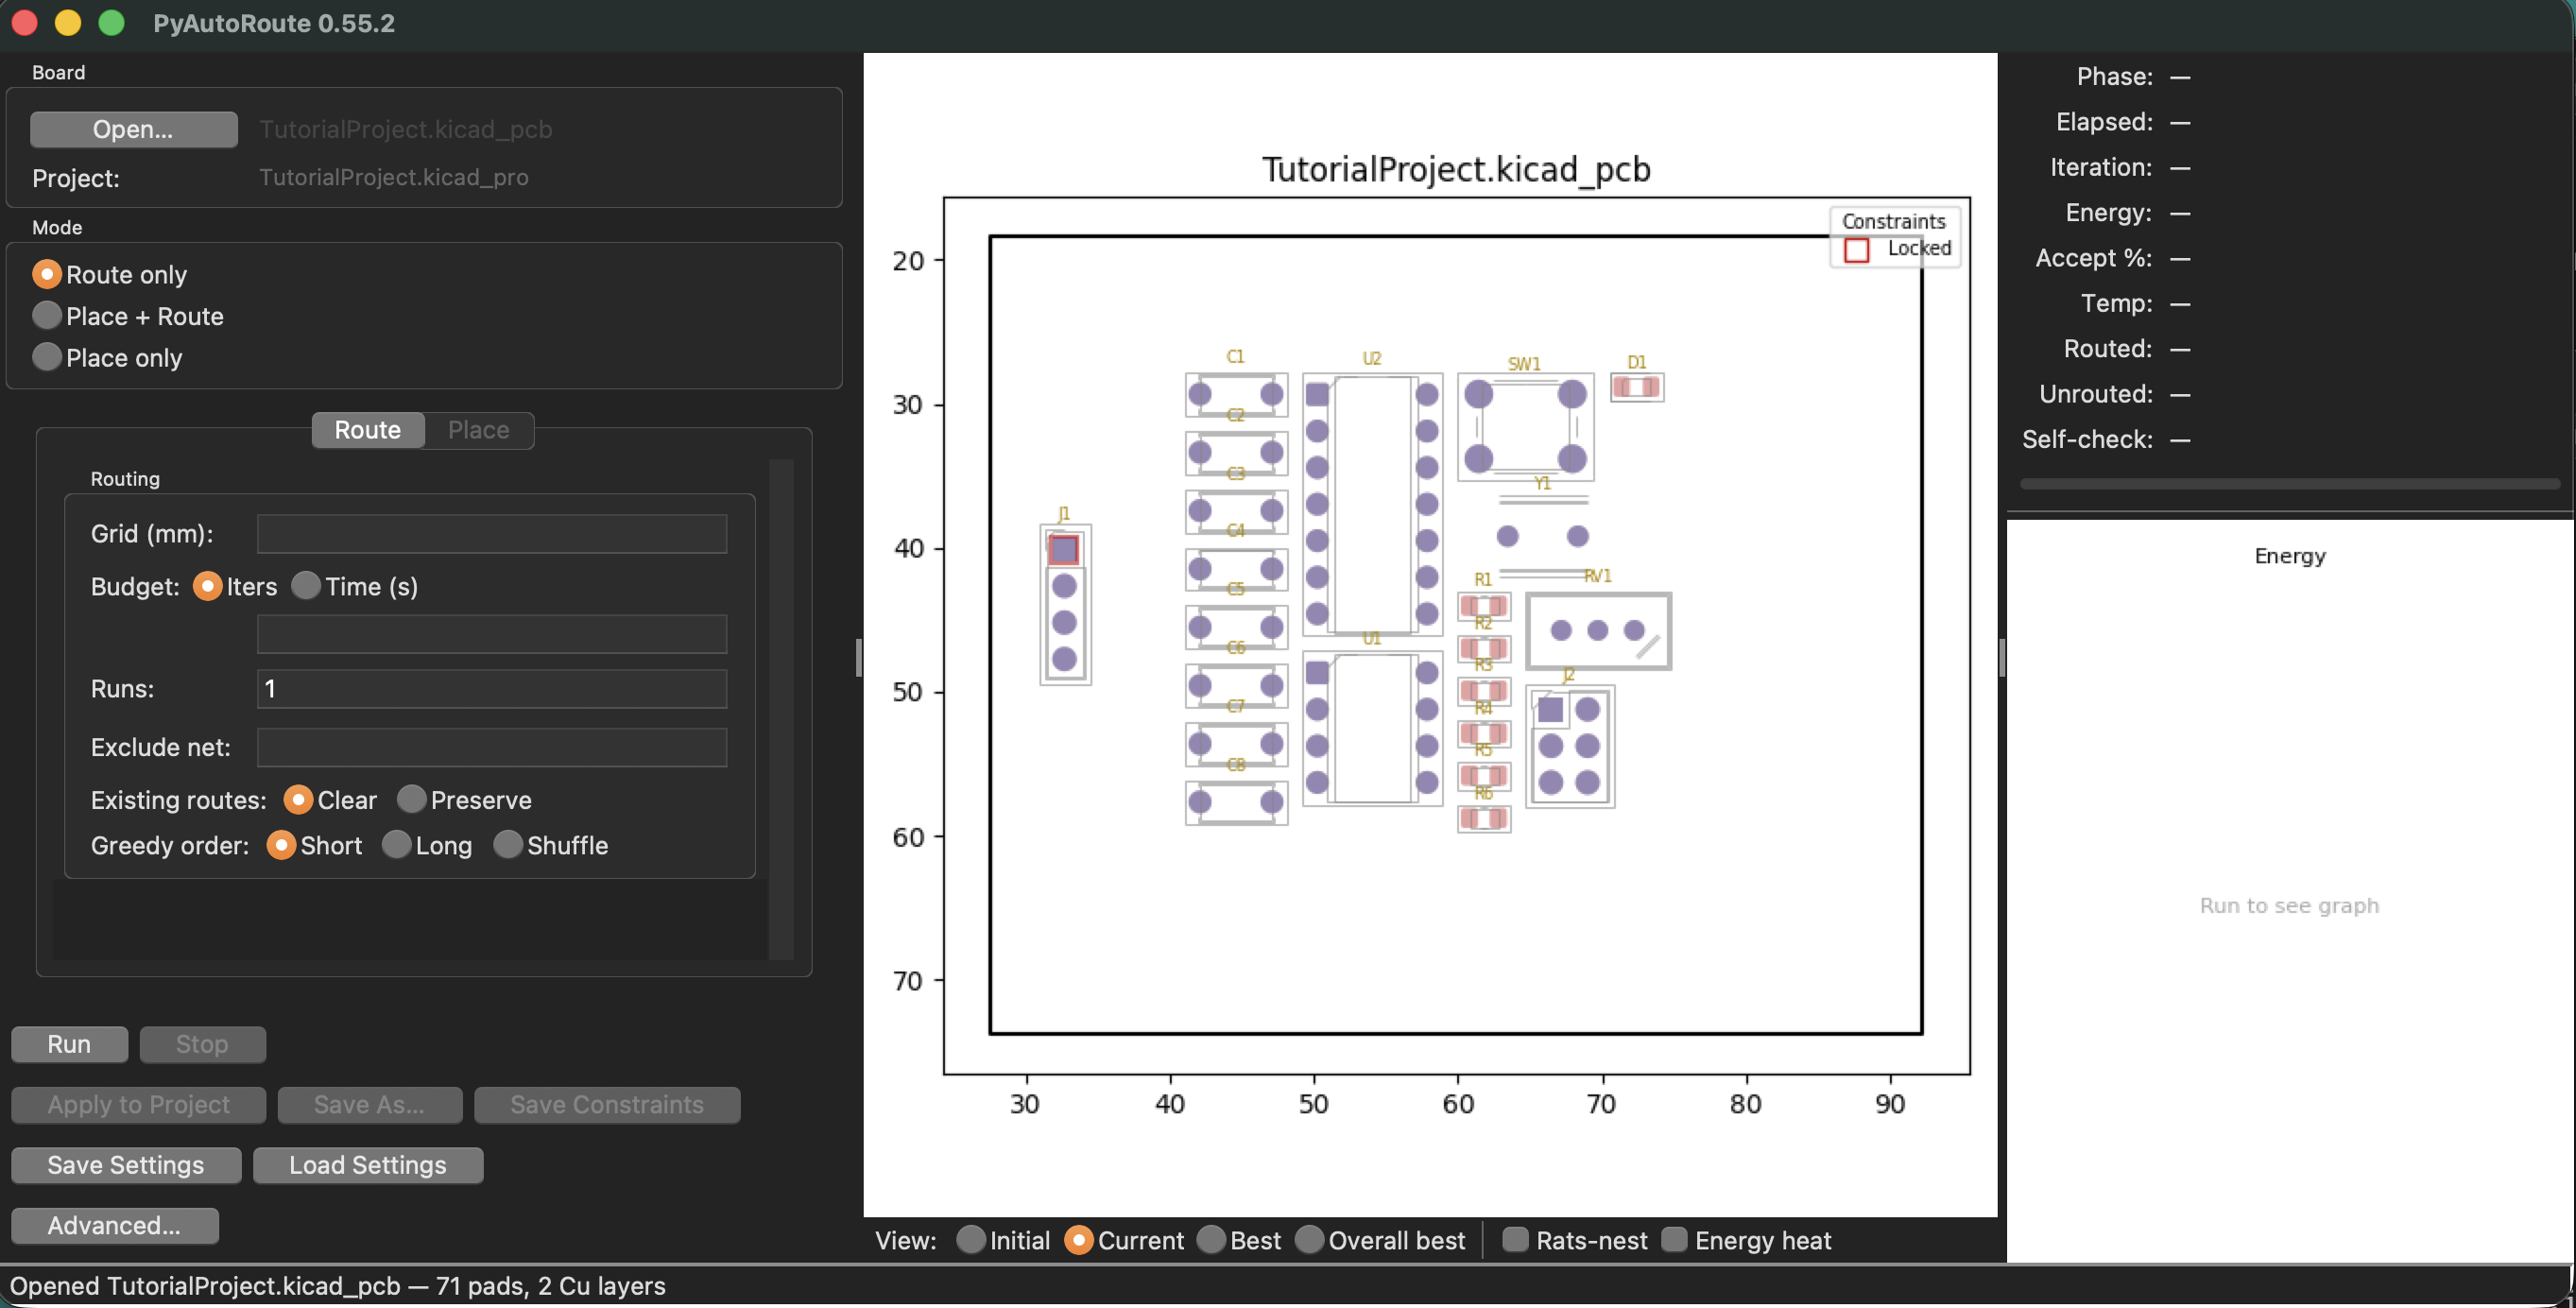
\includegraphics[width=\textwidth]{images/Gui Initial View.png}
    \caption{The PyAutoRoute GUI after opening the tutorial board.
             Controls are on the left, the board canvas in the centre,
             and live run statistics on the right.}
    \label{fig:gui-initial}
\end{figure}

\subsection{Setting footprint constraints}

Right-clicking any footprint on the canvas opens the constraint menu
(Figure~\ref{fig:gui-constraints}), with four options:

\begin{itemize}
    \item \textbf{Edge} --- attach the footprint to a board edge
          (\emph{Left}, \emph{Right}, \emph{Top}, \emph{Bottom}, or
          \emph{None}). The part is then pulled to that boundary during
          placement and oriented flat against it.
    \item \textbf{Lock} --- freeze the footprint's position so the
          placer treats it as a fixed obstacle.
    \item \textbf{Overlap OK} --- allow this footprint's body to
          overlap others (e.g.\ a shield sitting over the board).
    \item \textbf{Decoupling cap} --- pull a capacitor toward its
          associated IC during placement.
\end{itemize}

\begin{figure}[H]
    \centering
    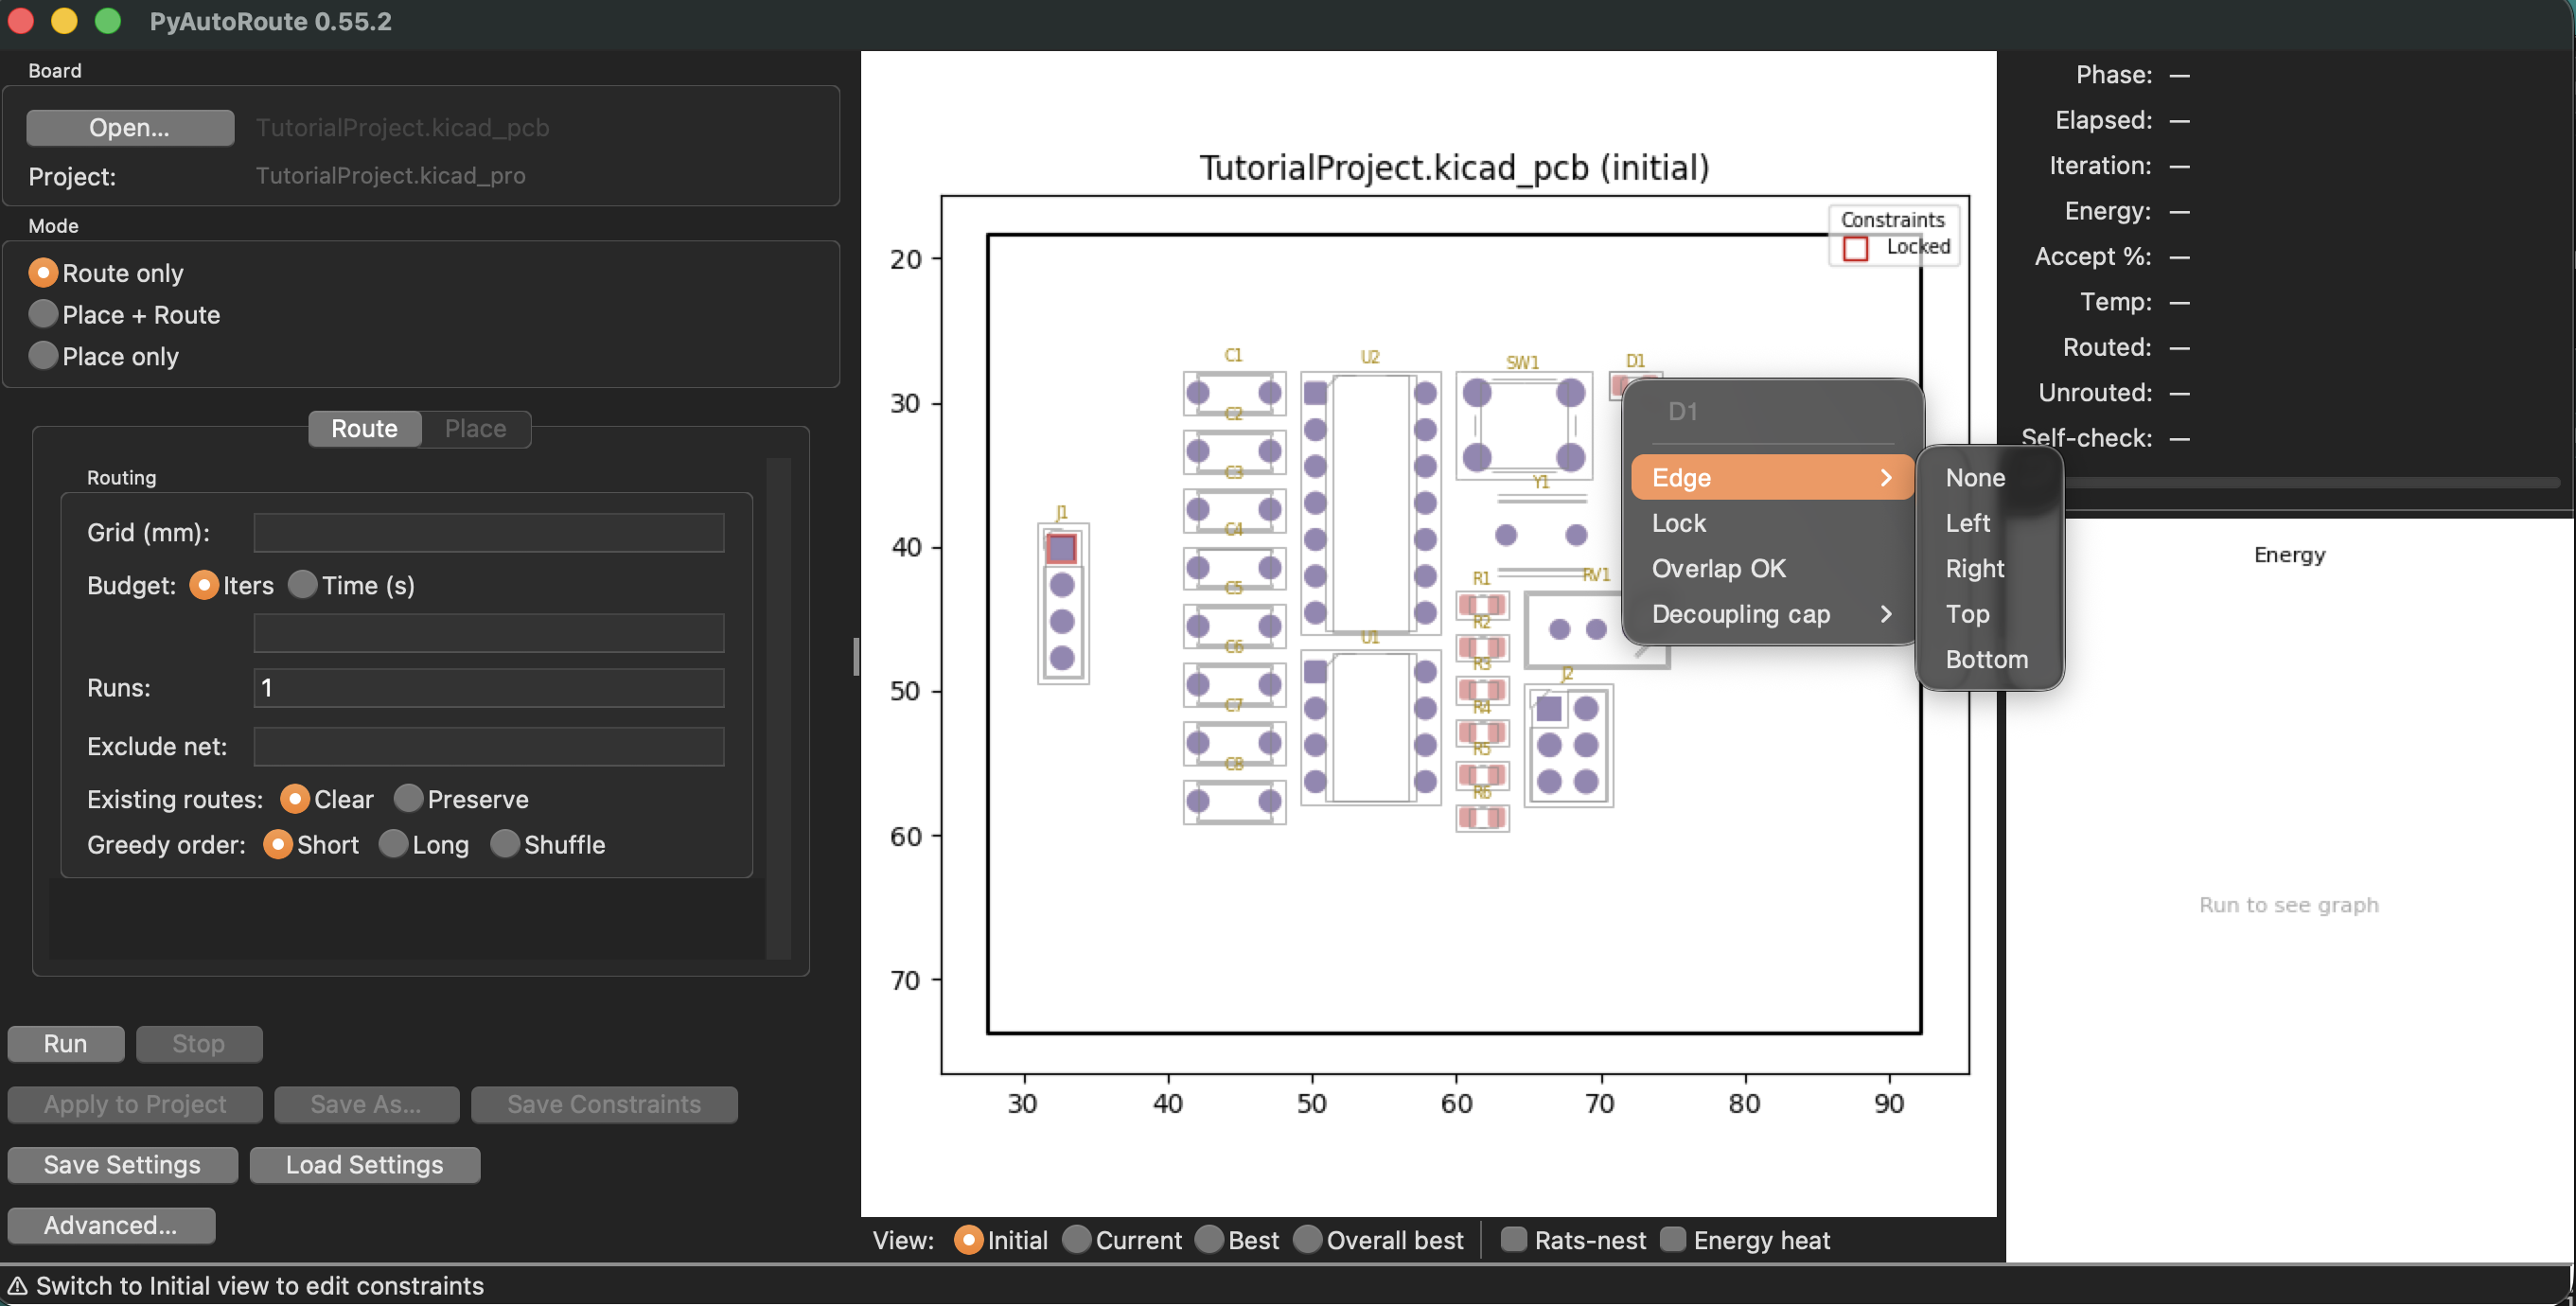
\includegraphics[width=\textwidth]{images/Setting footprint properties.png}
    \caption{Right-clicking \texttt{D1} (the LED) opens the constraint
             menu. Here the \emph{Edge} submenu is open, ready to attach
             the LED to a specific board boundary.}
    \label{fig:gui-constraints}
\end{figure}

For this tutorial, set \texttt{D1} to prefer the right edge
(\emph{Edge $\to$ Right}). The canvas immediately shows an orange arrow
on \texttt{D1} pointing toward the right boundary
(Figure~\ref{fig:gui-edge}), confirming the constraint is active.

\begin{figure}[H]
    \centering
    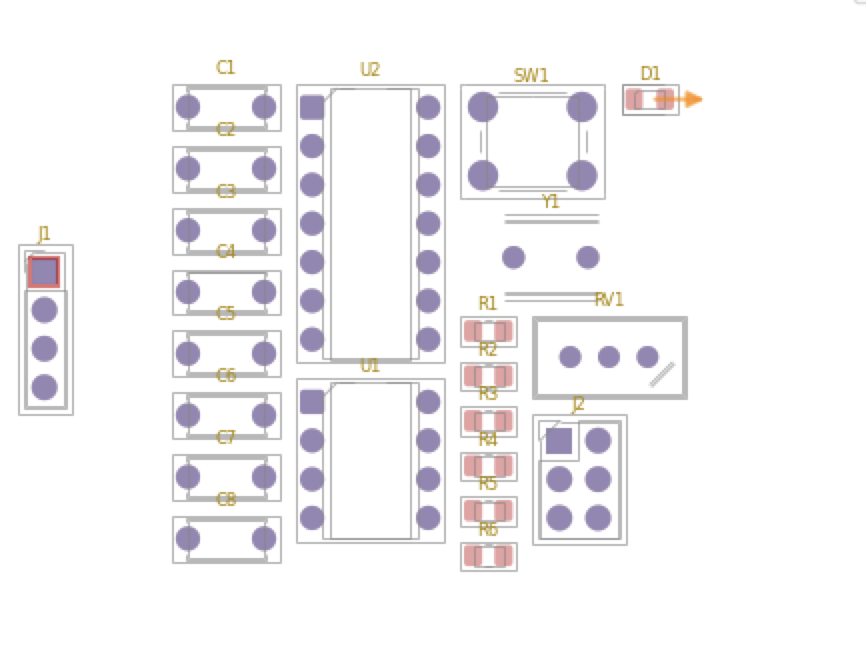
\includegraphics[width=0.8\textwidth]{images/Led prefer right edge.png}
    \caption{\texttt{D1} with an \emph{Edge = Right} constraint applied.
             The orange arrow indicates the target edge; the placer will
             pull the LED to the right boundary and orient it flat
             against it.}
    \label{fig:gui-edge}
\end{figure}

To lock the output connector \texttt{J1} in its current position,
right-click it and choose \emph{Lock}. Locked footprints are shown with
a distinctive highlight in the canvas (Figure~\ref{fig:gui-locked}) and
listed in the constraints legend (top-right of the canvas).

\begin{figure}[H]
    \centering
    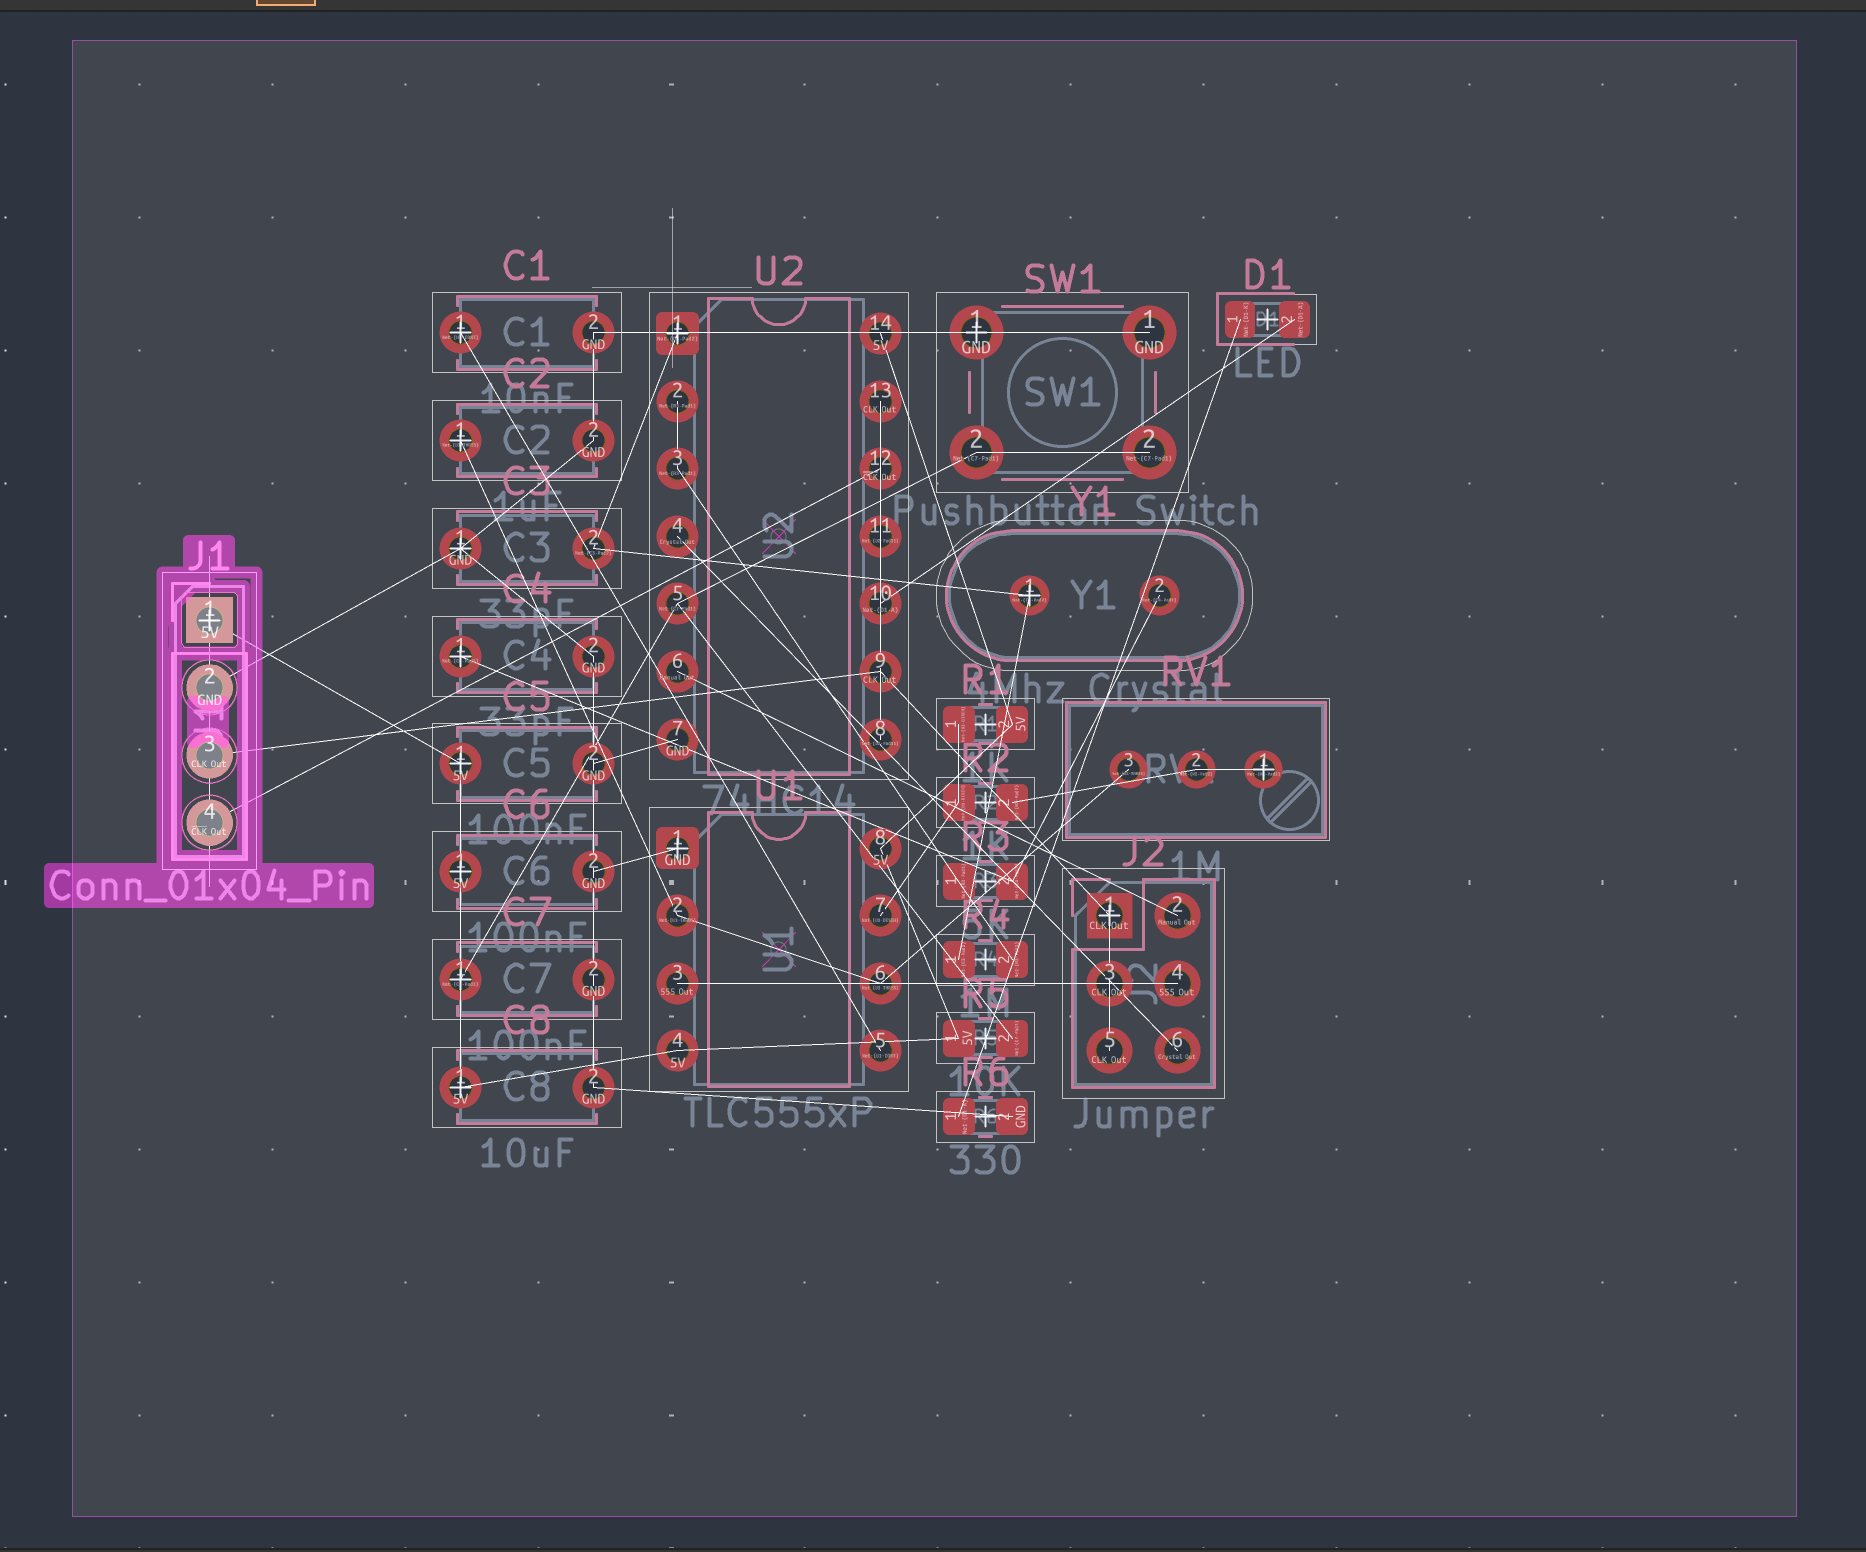
\includegraphics[width=0.7\textwidth]{images/Locked Component.png}
    \caption{\texttt{J1} locked in place. The placer will treat it as a
             fixed obstacle; all other footprints are arranged around it.}
    \label{fig:gui-locked}
\end{figure}

\subsection{Advanced settings}

Click \emph{Advanced\ldots} to open the full settings dialog
(Figure~\ref{fig:gui-advanced}). This exposes the placement and routing
energy weights, annealing schedule temperatures, post-processing options
(silk labels, ground plane, mounting holes), and the \textbf{Keep board
outline} toggle.

\begin{figure}[H]
    \centering
    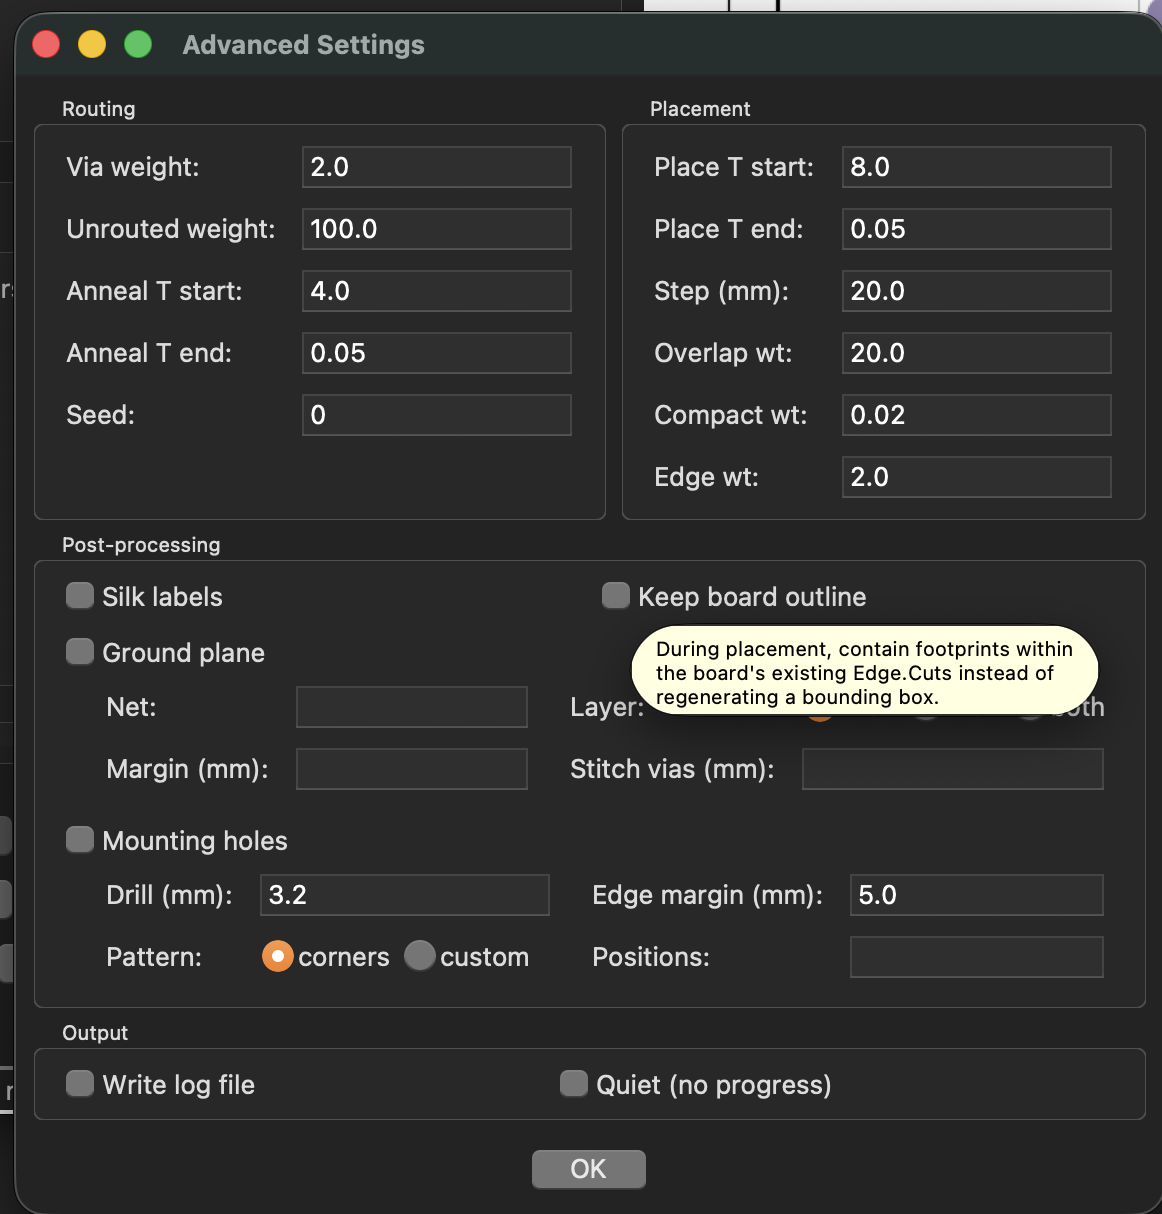
\includegraphics[width=0.7\textwidth]{images/Keep Board Outline.png}
    \caption{The Advanced Settings dialog. The \emph{Keep board outline}
             option (highlighted) constrains placement to the existing
             \texttt{Edge.Cuts} shape instead of regenerating a bounding
             rectangle --- useful when the board has a fixed mechanical
             outline.}
    \label{fig:gui-advanced}
\end{figure}

\subsection{Running placement}

Select \textbf{Place only} mode, set a time budget (60\,s is a good
starting point) and a run count of 3, then click \emph{Run}. The
annealer starts immediately; the energy graph on the right updates in
real time as the temperature cools and the placement converges.

Figure~\ref{fig:gui-placed} shows the result after three 60\,s runs.
The footprints are compactly arranged, \texttt{D1} has been pulled to
the right boundary as requested, \texttt{J1} is in its locked position,
and the self-check reads \textbf{PASS}.

\begin{figure}[H]
    \centering
    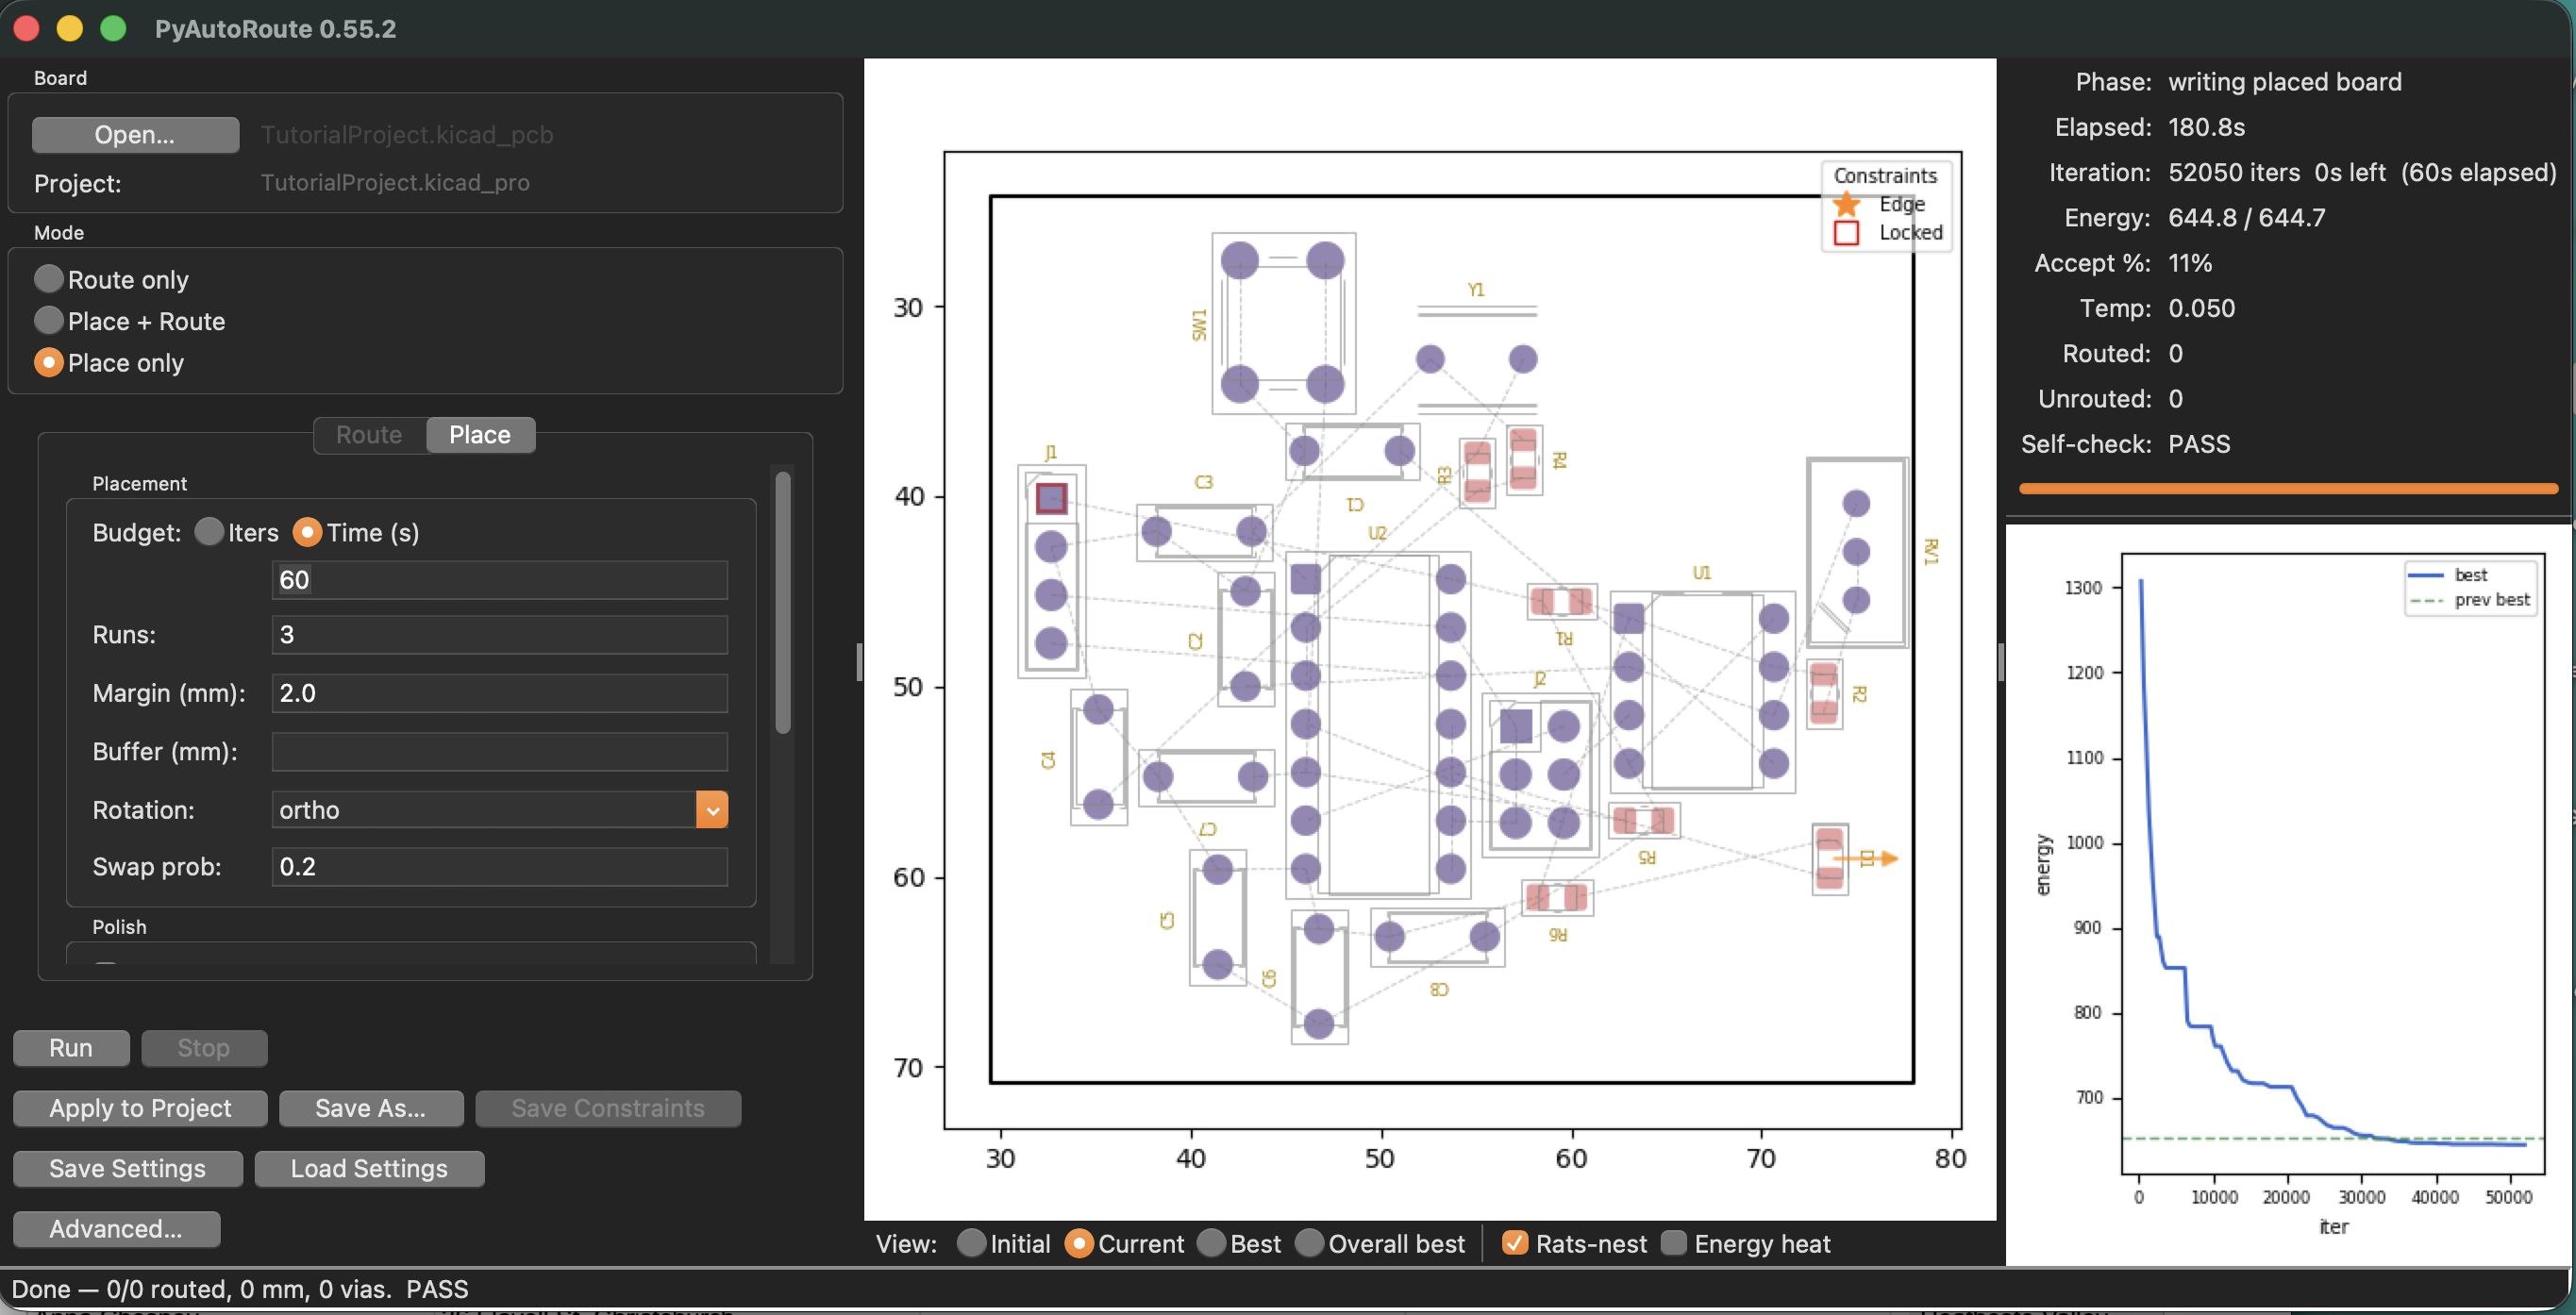
\includegraphics[width=\textwidth]{images/After Placing.png}
    \caption{After three placement runs of 60\,s each (180\,s total).
             The energy graph shows the annealer converging; the status
             panel confirms 0 unrouted connections and a clean
             self-check.}
    \label{fig:gui-placed}
\end{figure}

\subsection{Running the router}

Switch to \textbf{Route only} mode (the placed board is already in
memory), set a 30\,s time budget, and click \emph{Run} again. The
router completes the greedy pass and then anneals to reduce track
length and via count.

Figure~\ref{fig:gui-routed} shows the finished board: all 53
connections routed, 13 vias, 560\,mm total track length, and
Self-check: \textbf{PASS}. Click \emph{Save As\ldots} to write the
result to a \texttt{.kicad\_pcb} file, or \emph{Apply to Project} to
overwrite the project board in place.

\begin{figure}[H]
    \centering
    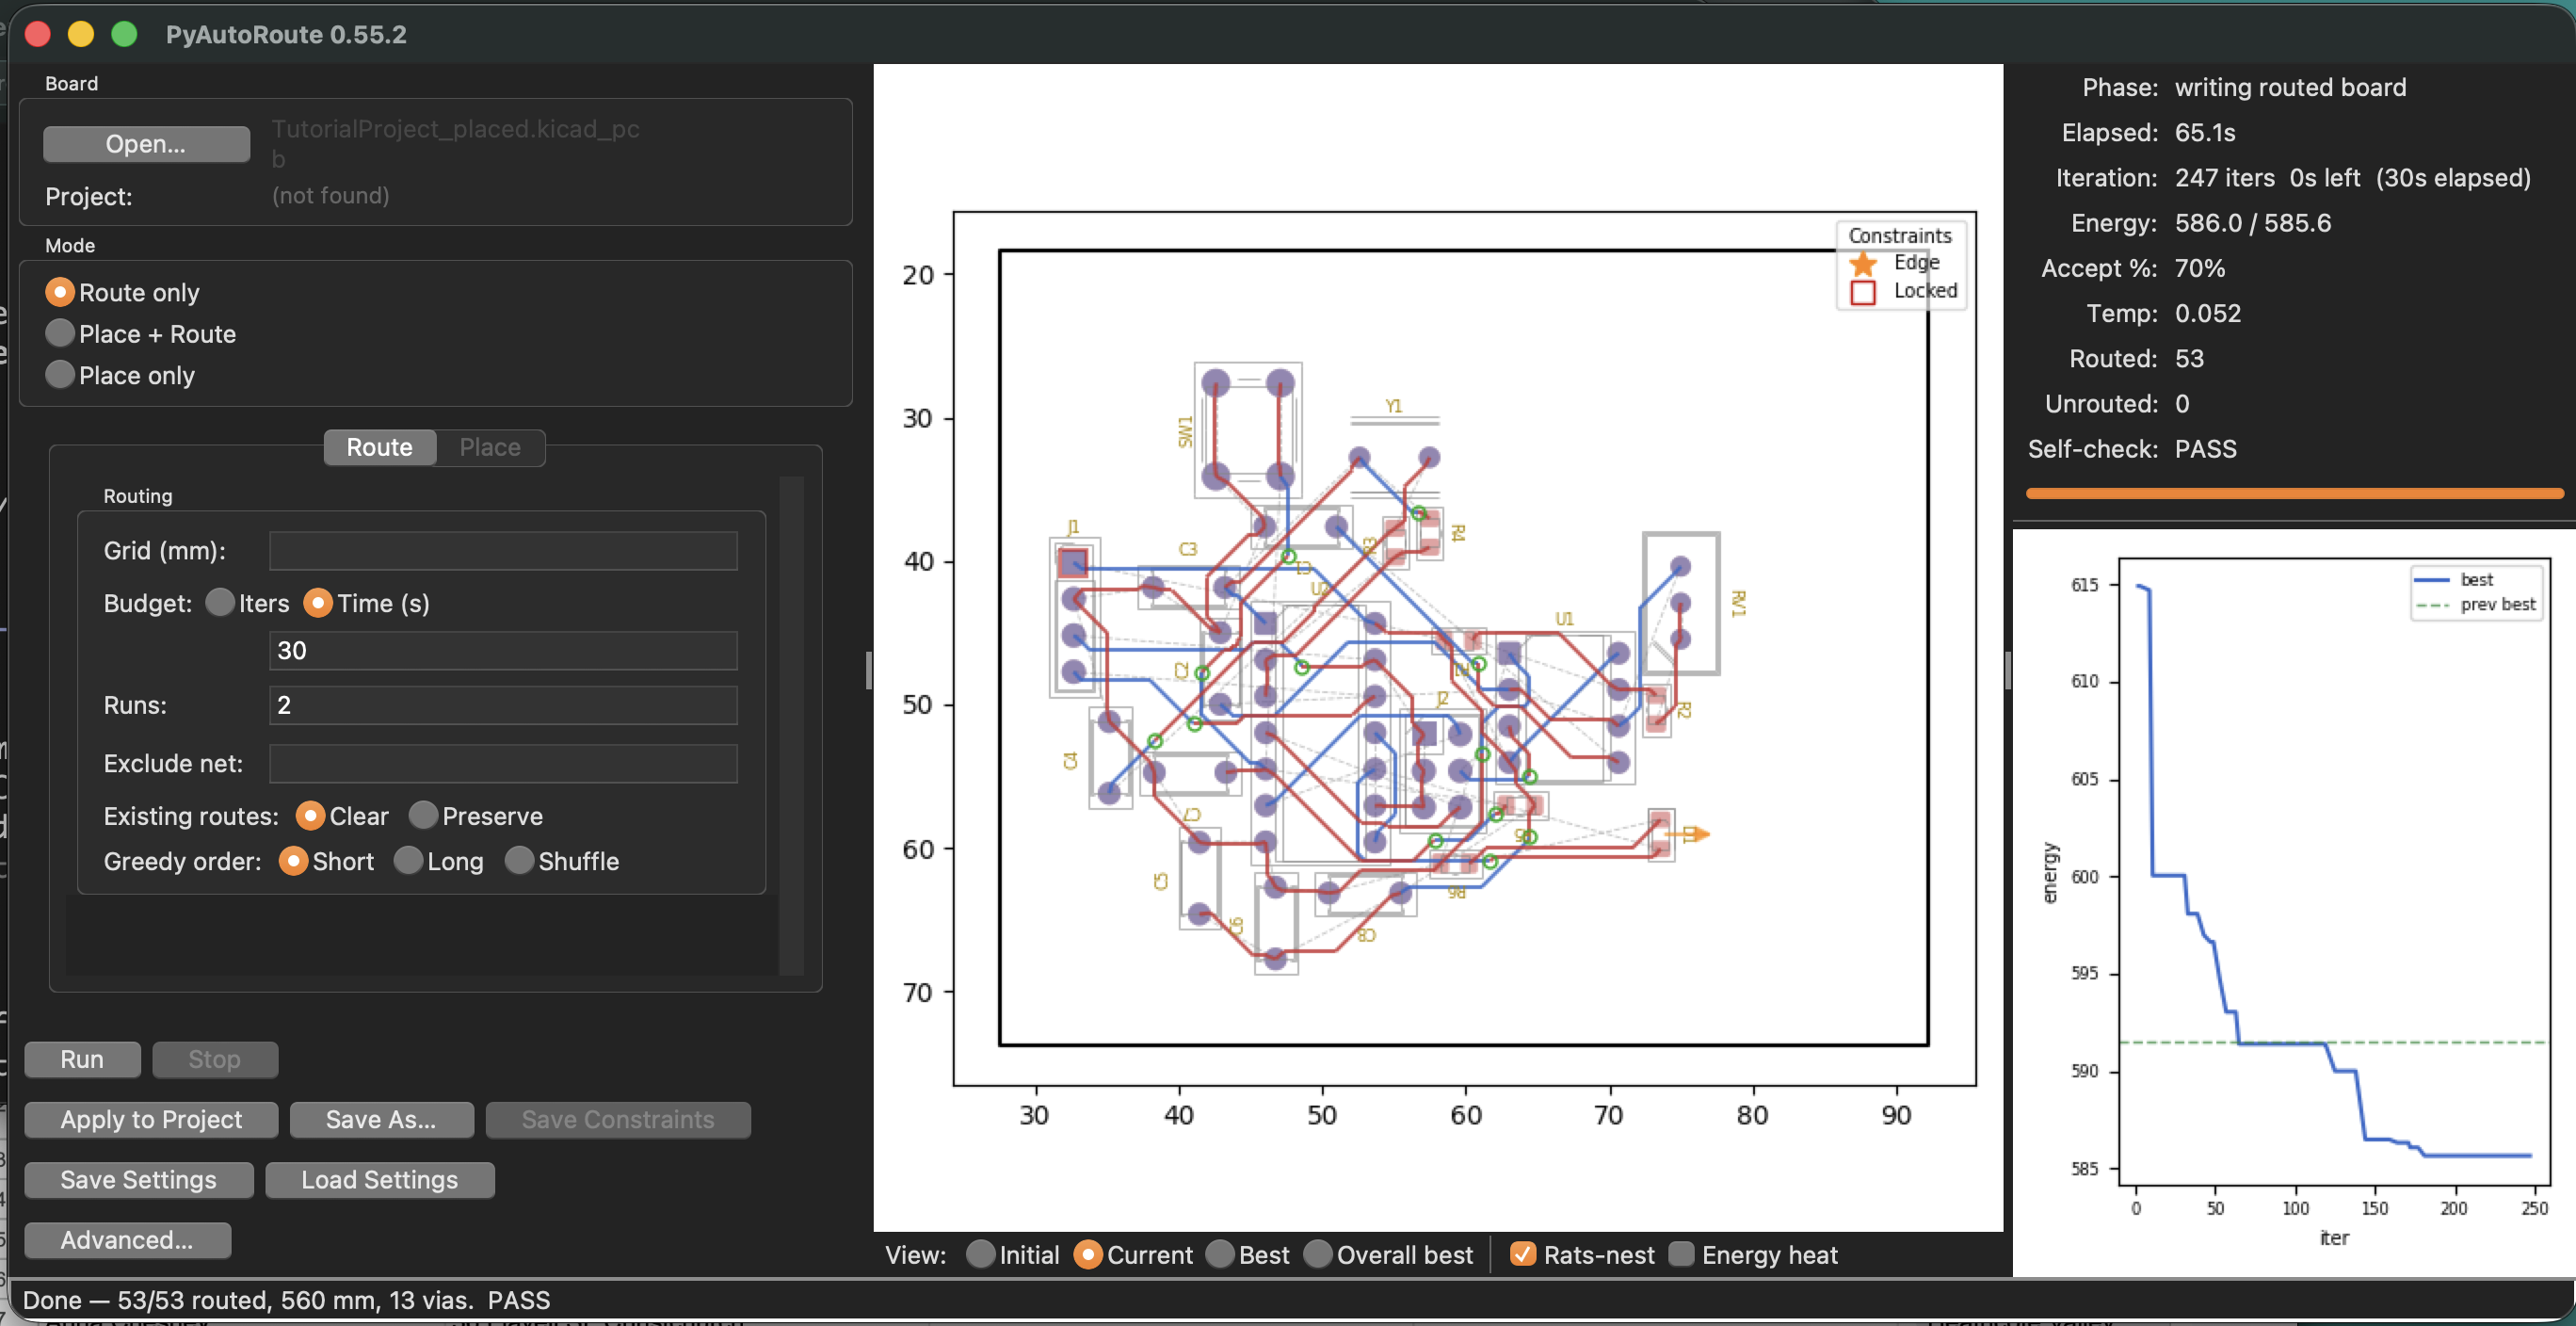
\includegraphics[width=\textwidth]{images/After Routing.png}
    \caption{The completed routed board. All 53 connections are routed
             (0 unrouted), with 13 vias and a clean self-check. The
             energy graph shows the annealing optimisation converging
             over the 30\,s budget.}
    \label{fig:gui-routed}
\end{figure}

% -----------------------------------------------------------------------
\section{Reviewing the Result}

Open the routed board in KiCad (\emph{File $\to$ Open}). Check:

\begin{enumerate}
    \item \textbf{DRC} --- run \emph{Inspect $\to$ Design Rules Checker}.
          Expect zero clearance violations; any ``unconnected'' items
          match the connections PyAutoRoute reported as unrouted.
    \item \textbf{Track inspection} --- use the 3D viewer
          (\emph{View $\to$ 3D Viewer}) to visually confirm track
          routing and layer usage.
    \item \textbf{Unrouted connections} --- if any remain, try a finer
          \texttt{--grid}, a longer \texttt{--routing-time}, or more
          \texttt{--runs}.
\end{enumerate}

PyAutoRoute also runs its own internal geometry self-check and reports
the result on the command line:

\begin{lstlisting}
  self-check:   clean (0 clearance violations)
  drill-check:  clean (0 hole-to-hole violations)
\end{lstlisting}

A non-zero exit code means a violation was found --- this should not
happen on a correctly set-up board, but the check provides an extra
safety net before you open KiCad.

% -----------------------------------------------------------------------
\section{Next Steps}

\begin{itemize}
    \item \textbf{Settings file} --- save your preferred options so
          you don't have to retype them:
\begin{lstlisting}
pyautoroute TutorialProject.kicad_pcb \
    --grid 0.2 --routing-time 60 --write-config
# creates TutorialProject.ini; next time just run:
pyautoroute TutorialProject.kicad_pcb
\end{lstlisting}
    \item \textbf{Ground plane} --- add \texttt{--ground-plane} to
          flood B.Cu with GND copper after routing. PyAutoRoute will
          call \texttt{kicad-cli} to fill the zone if it is installed.
    \item \textbf{KiCad plugin} --- install the plugin
          (\texttt{pyautoroute-install-plugin}) to run PyAutoRoute
          directly from the KiCad toolbar without leaving the editor.
    \item \textbf{Full documentation} --- see \texttt{README.md} and
          \texttt{docs/architecture.md} in the PyAutoRoute repository
          for the complete option reference and algorithm details.
\end{itemize}

% -----------------------------------------------------------------------
\section{Frequently Asked Questions}

% --- Routing problems ---------------------------------------------------
\subsection*{Some connections are still unrouted after routing. What should I try?}

Unrouted connections mean the A* search could not find a path --- usually
because the routing grid is too coarse to thread between closely-spaced
pads, or the annealing budget ran out before a global solution emerged.
Try these in order:

\begin{enumerate}
    \item \textbf{Finer grid} --- halve the grid pitch:
\begin{lstlisting}
pyautoroute board.kicad_pcb --grid 0.1
\end{lstlisting}
          A finer grid gives the router more room to manoeuvre around
          dense pad clusters, at the cost of a slower run.
    \item \textbf{Longer annealing budget} --- the rip-up/reroute loop
          needs time to untangle conflicting connections:
\begin{lstlisting}
pyautoroute board.kicad_pcb --routing-time 300
\end{lstlisting}
    \item \textbf{Multiple runs} --- annealing is stochastic; a different
          seed often finds a route the first seed missed:
\begin{lstlisting}
pyautoroute board.kicad_pcb --routing-time 60 --runs 5
\end{lstlisting}
    \item \textbf{Check pad clearances} --- if two pads sit closer
          together than the design-rule clearance, no router can pass
          copper between them. Open the board in KiCad and run DRC on
          the \emph{unrouted} board to catch physical conflicts before
          routing.
\end{enumerate}

% -----------------------------------------------------------------------
\subsection*{The routed board has too many vias. How do I reduce them?}

Each via costs \texttt{--via-weight} mm of equivalent track length in the
annealing energy (default 2.0). Raising this value makes the optimiser
treat vias as more expensive, so it works harder to stay on one layer:

\begin{lstlisting}
pyautoroute board.kicad_pcb --routing-time 60 --via-weight 8
\end{lstlisting}

Very high values (above~10) can make some nets unroutable if the only
path requires a layer change, so increase gradually. A complementary
approach is to prefer \texttt{F.Cu} with the default layer bias (already
built in) and use a finer grid so more single-layer paths become available.

% -----------------------------------------------------------------------
\subsection*{Routing is very slow on my board. How can I speed it up?}

Two knobs help:

\begin{itemize}
    \item \textbf{\texttt{--search-margin MM}} --- bounds each
          connection's A* search to a box around its endpoints, grown by
          \texttt{MM} on every side. The router widens the box and retries
          if it cannot find a route, ultimately falling back to the whole
          grid. This dramatically speeds up the rip-up/reroute loop on
          large or sparse boards:
\begin{lstlisting}
pyautoroute board.kicad_pcb --routing-time 120 --search-margin 10
\end{lstlisting}
    \item \textbf{Coarser grid} --- a 0.2\,mm or 0.25\,mm grid is
          significantly faster than 0.1\,mm and is sufficient for most
          hobby boards with 0.2\,mm clearance rules. Use
          \texttt{pyautoroute-tune} to find the best grid for your board
          automatically.
    \item \textbf{Parallel runs} --- combine \texttt{--runs N} with
          \texttt{--jobs 0} to use all CPU cores, keeping total wall-clock
          time the same while exploring more seeds:
\begin{lstlisting}
pyautoroute board.kicad_pcb --routing-time 60 --runs 8 --jobs 0
\end{lstlisting}
\end{itemize}

% --- Placement ----------------------------------------------------------
\subsection*{Components are overlapping after \texttt{-{}-place}. What is wrong?}

The placement annealer uses the \textbf{courtyard layer}
(\texttt{F.CrtYd} / \texttt{F.Courtyard}) to determine each
footprint's physical body extent. If a footprint in your KiCad library
is missing a courtyard, the placer falls back to the pad bounding box,
which can be much smaller than the actual body --- a common situation
with round electrolytic capacitors, whose two pads span only the lead
pitch while the body extends well beyond them.

To fix this:
\begin{itemize}
    \item Open the footprint editor in KiCad and add a
          \texttt{F.CrtYd} rectangle or circle that tightly encloses the
          physical body.
    \item Alternatively, increase \texttt{--place-buffer} to add extra
          clearance around all footprints, which compensates for a
          missing or undersized courtyard at the cost of a larger layout:
\begin{lstlisting}
pyautoroute board.kicad_pcb --place --place-buffer 2.0
\end{lstlisting}
\end{itemize}

% -----------------------------------------------------------------------
\subsection*{How do I keep a connector at the board edge?}

Add a footprint property named \texttt{Autoroute-edge} with value
\texttt{any} (nearest edge), or \texttt{left} / \texttt{right} /
\texttt{top} / \texttt{bottom} to pin a specific side. In KiCad:
\emph{Footprint Properties $\to$ Fields $\to$ +}, name
\texttt{Autoroute-edge}, value \texttt{right}.

The placer then pulls the footprint to that edge \emph{and} orients it
flat against the boundary, so all its pins lie near the board perimeter.
The pull strength is controlled by \texttt{--place-edge-weight} (default
2.0; higher pulls harder). Unlike locking, the footprint is still free
to slide along the edge while the rest of the layout optimises around it.

% -----------------------------------------------------------------------
\subsection*{How do I stop a specific component from moving during placement?}

Lock the footprint in KiCad (\emph{right-click $\to$ Lock}, or press
\texttt{L}). KiCad stores this as a \texttt{(locked yes)} attribute in
the \texttt{.kicad\_pcb} file, which PyAutoRoute reads and treats as a
fixed obstacle. Locked footprints are listed on startup so you can
confirm what is pinned before a run.

This is useful for mounting holes, edge-mount connectors, or any part
that must occupy an exact mechanical position.

% --- Workflow -----------------------------------------------------------
\subsection*{Where does PyAutoRoute write its output, and what are the file names?}

PyAutoRoute never modifies the input file (unless you pass
\texttt{--in-place}). Output naming follows the mode:

\begin{center}
\begin{tabular}{ll}
    \toprule
    \textbf{Mode} & \textbf{Output filename} \\
    \midrule
    Route only (default)        & \texttt{INPUT\_routed.kicad\_pcb} \\
    Place then route (\texttt{--place})   & \texttt{INPUT\_placed\_routed.kicad\_pcb} \\
    Place only (\texttt{--place-only})    & \texttt{INPUT\_placed.kicad\_pcb} \\
    \bottomrule
\end{tabular}
\end{center}

Use \texttt{-o PATH} to override the output path entirely.

% -----------------------------------------------------------------------
\subsection*{How do I re-run with the same settings without retyping them?}

Write the current settings to an INI file with \texttt{--write-config}:

\begin{lstlisting}
pyautoroute board.kicad_pcb --grid 0.15 --routing-time 120 \
    --via-weight 5 --write-config
\end{lstlisting}

This creates \texttt{board.ini} alongside the board. On every subsequent
run, PyAutoRoute auto-loads that file --- so you can just type:

\begin{lstlisting}
pyautoroute board.kicad_pcb
\end{lstlisting}

Command-line options always override the file, so you can still do
one-off experiments without editing it.

% -----------------------------------------------------------------------
\subsection*{Can I route a board that I have already partially routed by hand?}

Yes. Pass \texttt{--existing-routes preserve}:

\begin{lstlisting}
pyautoroute board.kicad_pcb --existing-routes preserve
\end{lstlisting}

PyAutoRoute keeps all existing copper, works out which connections it
already satisfies, and routes only the remainder --- treating the
existing tracks as fixed obstacles. This lets you hand-route critical
signals first and delegate the rest to the autorouter.

The default is \texttt{--existing-routes clear}, which strips all tracks
before routing so re-running never doubles copper.

% --- Limitations --------------------------------------------------------
\subsection*{Does PyAutoRoute support more than two copper layers?}

No. The current router uses exactly two layers: \texttt{F.Cu} (front)
and \texttt{B.Cu} (back). Four-layer or six-layer boards are not
supported. If your design requires inner layers for power planes or
high-density routing, you will need a different tool for those nets;
PyAutoRoute can still handle the signal routing on the two outer layers
if the inner-layer copper is treated as a fixed obstacle.

% -----------------------------------------------------------------------
\subsection*{Can it handle copper pours and ground planes?}

PyAutoRoute does not \emph{route} into copper pours, but it can
\textbf{add a GND pour} after routing with \texttt{--ground-plane}:

\begin{lstlisting}
pyautoroute board.kicad_pcb --ground-plane \
    --ground-plane-layer B.Cu --stitch-vias
\end{lstlisting}

This emits a zone boundary following the board outline on the chosen
layer. If \texttt{kicad-cli} is installed, PyAutoRoute fills the zone
automatically; otherwise open the board in KiCad and run
\emph{Edit $\to$ Fill All Zones} (\texttt{B}).

Existing filled copper zones in the input board are detected and
excluded from routing --- their net is not routed and the filled polygon
is not treated as an obstacle (KiCad fills them after the fact).

% -----------------------------------------------------------------------
\subsection*{Will PyAutoRoute handle impedance-controlled or high-speed signals correctly?}

Not automatically. PyAutoRoute minimises total track length and via count
but has no knowledge of:

\begin{itemize}
    \item \textbf{Controlled impedance} --- track width for a target
          impedance on a given stack-up must be set manually (use a fixed
          net-class width in KiCad; PyAutoRoute respects net-class rules).
    \item \textbf{Matched-length pairs} --- the router does not length-tune
          single-ended signals. Differential pairs (\texttt{--diff-pairs})
          are routed coupled with controlled gap, which helps impedance,
          but skew trimming is not performed.
    \item \textbf{Crosstalk, return-path continuity, EMC} --- none of
          these are modelled.
\end{itemize}

For low-frequency hobby boards (audio, microcontrollers, retrocomputer
logic) these limitations rarely matter. For RF, high-speed digital
(DDR, USB~3, PCIe), or safety-critical designs, use PyAutoRoute as a
starting point and review the critical nets manually before fabrication.

\end{document}
